% Journal-style version of the Experiment 2 report (layout modelled on a Cell Press
% research article). Filled from the processed results by R/08_assemble_reports.R;
% compiled with XeLaTeX. This is a course report typeset in a journal layout, not a
% journal publication.
\documentclass[9pt,twocolumn]{extarticle}
\usepackage[letterpaper,top=0.72in,bottom=0.85in,left=0.62in,right=0.62in,columnsep=0.27in,headsep=12pt,footskip=24pt]{geometry}
\usepackage{fontspec}
\setmainfont{Liberation Sans}[Scale=0.96]
\newfontfamily\dejavu{DejaVu Sans}[Scale=0.9]
\usepackage{xcolor}
\definecolor{cellblue}{RGB}{0,99,155}
\definecolor{inkgrey}{RGB}{70,70,70}
\definecolor{rulegrey}{RGB}{150,150,150}
\definecolor{lav}{RGB}{244,241,250}
\usepackage{graphicx,booktabs,array,tabularx,colortbl,multirow,url}
\usepackage{caption}
\captionsetup{font={footnotesize},labelfont={bf},labelsep=period,justification=justified,singlelinecheck=false,skip=5pt}
\usepackage{titlesec}
\titleformat{\section}{\bfseries\fontsize{9.5}{11}\selectfont}{}{0pt}{\MakeUppercase}
\titlespacing*{\section}{0pt}{10pt}{3pt}
\titleformat{\subsection}{\bfseries\fontsize{9}{11}\selectfont}{}{0pt}{}
\titlespacing*{\subsection}{0pt}{7pt}{2pt}
\titleformat{\subsubsection}[runin]{\bfseries}{}{0pt}{}[]
\titlespacing*{\subsubsection}{0pt}{5pt}{5pt}
\usepackage{fancyhdr}
\usepackage{dblfloatfix}
\usepackage{enumitem}
\usepackage[hidelinks]{hyperref}
\hypersetup{pdftitle={Kinetics of Escherichia coli beta-galactosidase with ONPG and its inhibition by IPTG (B241 Experiment 2, journal-style version)},pdfauthor={Almokhtar Aljarodi}}
\usepackage{microtype}
\setlength{\parindent}{9pt}\setlength{\parskip}{0pt}
\linespread{1.06}
\newcommand{\cit}[1]{\textsuperscript{#1}}
\newcommand{\Km}{\textit{K}\textsubscript{m}}
\newcommand{\Kmapp}{\textit{K}\textsubscript{m,app}}
\newcommand{\Vmax}{\textit{V}\textsubscript{max}}
\newcommand{\Vmaxapp}{\textit{V}\textsubscript{max,app}}
\newcommand{\Vo}{\textit{V}\textsubscript{0}}
\newcommand{\Ki}{\textit{K}\textsubscript{i}}
\newcommand{\Kip}{\textit{K}\textsubscript{i}′}
\newcommand{\kcat}{\textit{k}\textsubscript{cat}}
\newcommand{\Rsq}{\textit{R}\textsuperscript{2}}
\newcommand{\Aa}{\textit{A}\textsubscript{415}}
\newcommand{\dAa}{Δ\textit{A}\textsubscript{415}}
\newcommand{\permin}{min\textsuperscript{−1}}
\newcommand{\umolmin}{µmol min\textsuperscript{−1}}
\newcommand{\epsunits}{mM\textsuperscript{−1} cm\textsuperscript{−1}}
\newcommand{\Ecoli}{\textit{Escherichia coli}}
\newcommand{\ecoli}{\textit{E. coli}}
\newcommand{\lac}{\textit{lac}}
\newcommand{\lacZ}{\textit{lacZ}}
\newcommand{\onp}{\textit{o}-nitrophenol}
\newcommand{\starsym}{{\dejavu ★}}
\newcommand{\ghead}[1]{\vspace{2pt}{\bfseries #1}\par\vspace{2pt}}
\newcommand{\dash}{–}
\renewcommand{\arraystretch}{1.15}
\pagestyle{fancy}\fancyhf{}
\renewcommand{\headrulewidth}{0.4pt}\renewcommand{\headrule}{\vspace{-2pt}{\color{rulegrey}\hrule width\headwidth height 0.4pt}}
\fancyhead[L]{\footnotesize\bfseries\color{cellblue}Article}
\fancyhead[R]{\footnotesize\color{inkgrey}Journal-style course report \textbar{} B241 Methods in Molecular and Cellular Biology, KAUST}
\fancyfoot[L]{\footnotesize\color{inkgrey}Experiment 2, \textit{o}-nitrophenyl-β-D-galactopyranoside kinetics, 11 October 2026}
\fancyfoot[R]{\footnotesize\color{inkgrey}\thepage}
\renewcommand{\footrulewidth}{0pt}

\begin{document}

% ------------------------------------------------------------------ highlights page
\onecolumn
\thispagestyle{fancy}
\vspace*{2pt}
{\footnotesize\bfseries\color{cellblue}Article}\par\vspace{6pt}
{\fontsize{19}{23}\selectfont\bfseries\raggedright Stopped-reaction kinetics of \ecoli{} β-galactosidase with ONPG: substrate saturation and inhibition by IPTG consistent with a competitive mechanism\par}
\vspace{14pt}
\ghead{Graphical abstract}
\begin{center}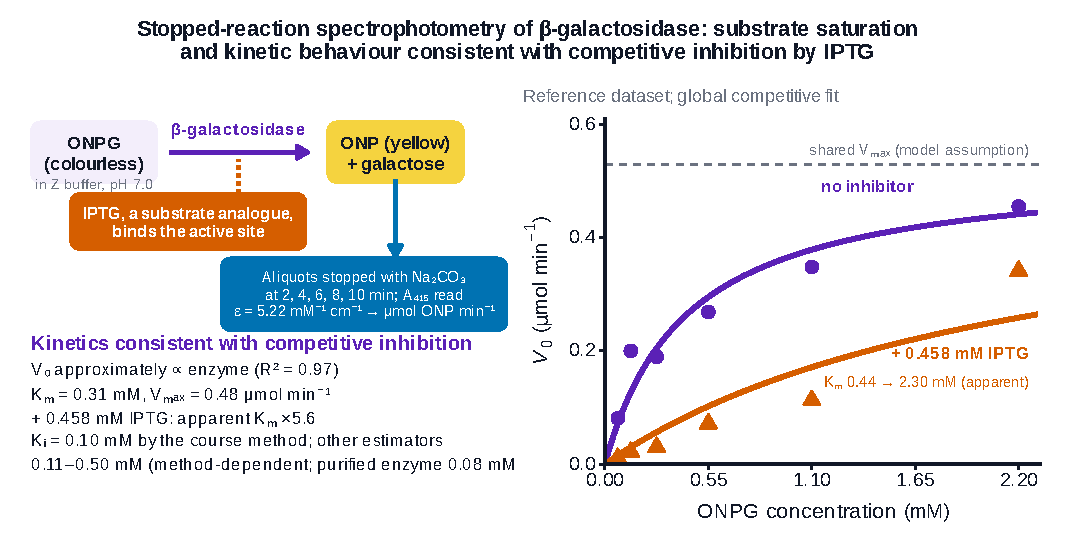
\includegraphics[width=0.96\textwidth]{../../figures/graphical_abstract.pdf}\end{center}
\vspace{10pt}
\noindent\begin{minipage}[t]{0.47\textwidth}
\ghead{Highlights}
\begin{itemize}[leftmargin=10pt,itemsep=3pt,topsep=0pt,label=\textbullet]
\item ONP calibration at 415 nm (ε = 5.22 \epsunits) converts absorbance rates to product formed
\item β-Galactosidase velocity rises approximately with enzyme amount and saturates with ONPG (\Km{} ≈ 0.3\dash 0.6 mM)
\item IPTG raises the apparent \Km{} 5.6-fold; a competitive model fits both series better than a noncompetitive one
\item \Ki{} = 0.10 mM by the course method; alternative estimators give 0.11\dash 0.50 mM (method-dependent estimates, not a confidence interval), the same order as the purified-enzyme value
\end{itemize}
\vspace{10pt}
\ghead{Authors}
Almokhtar Aljarodi, Abdulrahman Khardali\par
\vspace{10pt}
\ghead{Correspondence}
almokhtaraljarodi@gmail.com\par
\end{minipage}\hfill
\begin{minipage}[t]{0.47\textwidth}
\ghead{In brief}
Using a stopped-reaction assay with the chromogenic substrate ONPG and a course-provided reference dataset, the authors measure the Michaelis constant and limiting velocity of \ecoli{} β-galactosidase and show that the \lac{} inducer IPTG raises the apparent \Km{} and inhibits most where substrate is lowest, kinetic behaviour consistent with competitive inhibition, with a \Ki{} of the same order as that of the purified enzyme. A single explicit rule for choosing initial-rate windows makes every velocity reproducible from the raw absorbances, and a sensitivity analysis shows which conclusions survive alternative rules and which, including the numerical \Ki, do not.
\end{minipage}
\vfill
{\footnotesize\color{inkgrey}Aljarodi \& Khardali, 11 October 2026, Journal-style course report, Experiment 2 (B241), King Abdullah University of Science and Technology. Layout modelled on a Cell Press research article; this document is a course report, not a journal publication.}
\clearpage

% ------------------------------------------------------------------ main text
\twocolumn[
\begin{@twocolumnfalse}
\vspace*{2pt}
{\footnotesize\bfseries\color{cellblue}Article}\par\vspace{6pt}
{\fontsize{19}{23}\selectfont\bfseries\raggedright Stopped-reaction kinetics of \ecoli{} β-galactosidase with ONPG: substrate saturation and inhibition by IPTG consistent with a competitive mechanism\par}
\vspace{10pt}
{\fontsize{10}{12}\selectfont\bfseries Almokhtar Aljarodi\textsuperscript{1,2,3,*} and Abdulrahman Khardali\textsuperscript{1}\par}
\vspace{5pt}
{\footnotesize
\textsuperscript{1}Methods in Molecular and Cellular Biology (B241), Biological and Environmental Science and Engineering Division, King Abdullah University of Science and Technology (KAUST), Thuwal, Saudi Arabia\\
\textsuperscript{2}M.S. Bioscience program, KAUST, Thuwal, Saudi Arabia\\
\textsuperscript{3}Lead contact\\
*Correspondence: almokhtaraljarodi@gmail.com\\
Code and data: see data and code availability\par}
\vspace{12pt}
\end{@twocolumnfalse}
]

\section{Summary}
Enzyme kinetics condenses how an enzyme responds to substrate, inhibitors and its own abundance into two constants, \Km{} and \Vmax. Here we characterize \Ecoli{} β-galactosidase acting on \textit{o}-nitrophenyl-β-D-galactopyranoside (ONPG) by stopped-reaction spectrophotometry, following the product \onp{} at 415 nm after quenching timed aliquots with Na\textsubscript{2}CO\textsubscript{3}. The primary kinetic analysis uses a course-provided reference dataset; measurements collected by our own group form an experimental dataset analyzed separately. A Beer\dash Lambert calibration (ε = 5.22 \epsunits) converts absorbance rates into product formed. Initial velocity rose approximately in proportion to enzyme concentration, and velocity saturated with ONPG (\Km{} = 0.31\dash0.36 mM, \Vmax{} = 0.48\dash0.49 \umolmin{} per assay). The gratuitous \lac{} inducer isopropyl-β-D-thiogalactopyranoside (IPTG) raised the apparent \Km{} 5.6-fold and inhibited most where substrate was lowest; a competitive model fitted both series with a residual sum of squares 1.9 times smaller than a pure noncompetitive model, behaviour consistent with competitive inhibition. \Ki{} depends on the model and on how initial rates are estimated from 2-min samples (0.10\dash0.22 mM across rule-based estimators), the same order as the 0.08 mM reported for the purified enzyme. An explicit rule for initial-rate windows makes every velocity reproducible from the raw absorbances.

\section{Introduction}
Enzymes accelerate reactions by binding substrates at active sites, and the dependence of velocity on substrate concentration reveals how tightly and how productively they do so. Michaelis and Menten described this dependence with a reversible enzyme\dash substrate complex that breaks down to product, giving \Vo{} = \Vmax[S]/(\Km{} + [S]).\cit{1,2} \Vmax{} = \kcat[E]\textsubscript{T} is the limiting velocity when every active site is occupied, and is therefore proportional to the amount of enzyme; \Km{} is the substrate concentration at half-maximal velocity and reports how much substrate is needed to engage the enzyme. Lineweaver and Burk rearranged the equation into a straight line, 1/\Vo{} = (\Km/\Vmax)(1/[S]) + 1/\Vmax, whose intercepts give the two constants.\cit{3} The reciprocal transform distorts the error structure of the data,\cit{4} but it remains the standard teaching representation; we report it alongside a direct fit of the untransformed data.

β-Galactosidase (EC 3.2.1.23), the \lacZ{} product of \Ecoli, is a homotetramer of 1023-residue subunits that hydrolyzes the β-1,4 glycosidic bond of lactose and of synthetic β-galactosides.\cit{5,6} The chromogenic substrate ONPG is cleaved to galactose and \onp. At alkaline pH, \onp{} exists as the yellow \textit{o}-nitrophenolate anion, whose absorbance near 415\dash 420 nm follows the Beer\dash Lambert law. Adding 1 M Na\textsubscript{2}CO\textsubscript{3} to a timed aliquot therefore both stops the reaction, by raising the pH far above the enzyme's working range, and develops the color, so one reading gives the product formed up to that moment.\cit{7} A series of stopped samples builds a progress curve whose initial slope is the initial velocity \Vo, measured before substrate depletion, product accumulation, or enzyme instability slow the reaction.

Inhibitors reveal themselves by how they change \Km{} and \Vmax. A competitive inhibitor binds free enzyme at the active site and is displaced by substrate: it leaves \Vmax{} unchanged but raises the apparent Michaelis constant to \Kmapp{} = \Km(1 + [I]/\Ki), where \Ki{} is the inhibitor's dissociation constant. A noncompetitive inhibitor inactivates a fraction of the enzyme whatever the substrate concentration, lowering \Vmax{} and leaving \Km{} unchanged.\cit{2} IPTG is the thiogalactoside used as a gratuitous inducer of the \lac{} operon because it induces the enzyme without being hydrolyzed by it.\cit{8,9} The same stability makes it a dead-end ligand of β-galactosidase: it occupies the galactose subsite of the active site, but its thioglycosidic bond is not cleaved, so it is expected to behave as a competitive inhibitor with a \Ki{} of the order of 0.1 mM.\cit{6,10}

Here we establish the ONP absorption spectrum and standard curve, measure the dependence of \Vo{} on enzyme concentration at saturating ONPG, and measure \Vo{} over a 32-fold range of ONPG concentrations with and without IPTG. Because five of the six uninhibited progress curves had already begun to decelerate within the first sampling interval, we formalized the choice of initial-rate window as an explicit, reproducible rule, tested its origin assumption, and quantified how much each kinetic constant depends on it.

\section{Results}

\subsection{ONP absorbs maximally at 415 nm and calibrates absorbance to product}
The spectrum of 0.333 mM ONP in the alkaline assay matrix peaked at 415 nm (\textit{A} = 1.723), with 410\dash 420 nm within 2\% of the maximum (Figure 1A), so 415 nm was used for all kinetic measurements. The course's standard-curve table listed seven readings against tubes 1\dash 7 while the manual describes a blank and seven standards; the first reading (0) is the zero-concentration preparation, as the instructor confirmed, and the remaining six were assigned to the manual's standards 1\dash 6, an assignment anchored by the spectrum tube (manual standard 4, which read 1.723 at 415 nm, identical to the fifth reading; Table S1). The manual's standard 7 (0.667 mM) has no reported reading and no value was assumed for it. Standards of 0.083\dash 0.433 mM ONP gave a linear Beer\dash Lambert plot, \Aa{} = 5.222[ONP] − 0.022 (\Rsq{} = 0.9988, \textit{n} = 5); the 0.533 mM standard (\textit{A} = 3.24) lay 17\% above the line and was excluded (Figure 1B). The slope gives ε = 5.22 ± 0.10 \epsunits{} (5222 M\textsuperscript{−1} cm\textsuperscript{−1}; 5.15 through the origin); including the excluded standard would give 6.01 \epsunits{} and lower every \Vmax{} by 13\% without affecting \Km{} or \Ki. The excluded reading transmits 0.06\% of the incident light, within but near the instrument's specified linear range (up to 3.5 A at 260 nm);\cit{13} because the deviation is upward, the opposite of stray-light saturation, its cause cannot be identified from a single reading. Every velocity below was converted with ε: a rate of 0.132 \dAa{} \permin{} (tube A, no inhibitor) corresponds to 0.132/5.22 = 0.0253 mM \permin{} in the cuvette, × 1.5 (stop dilution) = 0.0379 mM \permin{} in the reaction, × 12.0 mL = 0.455 µmol ONP \permin{} per assay.

\begin{figure*}[!tb]
\centering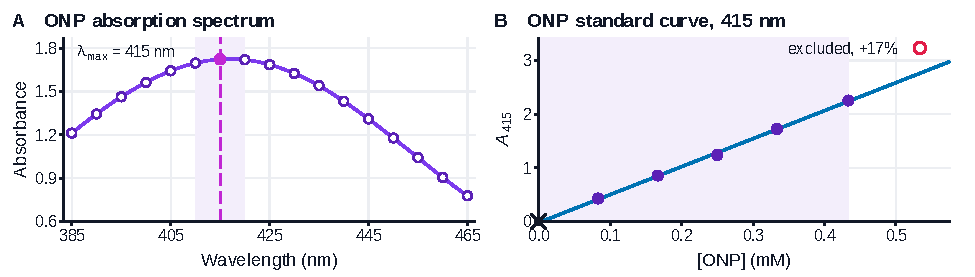
\includegraphics[width=\textwidth]{../../figures/figure1_onp_calibration.pdf}
\caption{\textbf{\onp{} absorbs maximally at 415 nm and obeys the Beer\dash Lambert law to 0.43 mM}\newline
(A) Absorbance spectrum of 0.333 mM ONP (1.0 mL of 1 mM ONP + 1.0 mL Z buffer + 1.0 mL 1 M Na\textsubscript{2}CO\textsubscript{3}) read from 465 to 385 nm in 5 nm steps against the Z buffer/Na\textsubscript{2}CO\textsubscript{3} blank. Points are readings, the line a spline, the dashed line the maximum at 415 nm (labeled); the shaded band (410\dash 420 nm) lies within 2\% of the maximum.\newline
(B) Standard curve at 415 nm for 1 mM ONP diluted to 0.083\dash 0.533 mM in the same 3.0 mL matrix. Filled points and the line are the least-squares calibration over the linear region (shaded): \Aa{} = 5.222[ONP] − 0.022, \Rsq{} = 0.9988, \textit{n} = 5, ε = 5.22 ± 0.10 \epsunits. ×, zero-concentration point (not fitted). The 0.533 mM standard (open, labeled) lay 17\% above the line and was excluded. Reference dataset, Part I; see STAR Methods.}
\end{figure*}

\subsection{Initial velocity scales approximately with enzyme concentration}
With 2.20 mM ONPG, product formation was linear over an initial window at every enzyme level (Figure 2A). \Vo{} fell from 0.469 \umolmin{} (0.136 \dAa{} \permin) with the undiluted enzyme to 0.079 \umolmin{} at 0.15 of that amount, a 5.9-fold change for a 6.7-fold dilution; relative rates were 1.00, 0.77, 0.60, 0.18, 0.17 for relative enzyme 1.00, 0.75, 0.50, 0.25, and 0.15. A line through the origin, \Vo{} = 0.481 × \textit{E} \umolmin, described the data with \Rsq{} = 0.972, and a free intercept was indistinguishable from zero (\textit{p} = 0.98; Figure 2B). The trend is approximately but not exactly proportional: the rate per unit enzyme ranged from 0.71 (tube D) to 1.21 (tube C), and tubes D and E (0.25 and 0.15) gave nearly equal rates.

\begin{figure*}[!tb]
\centering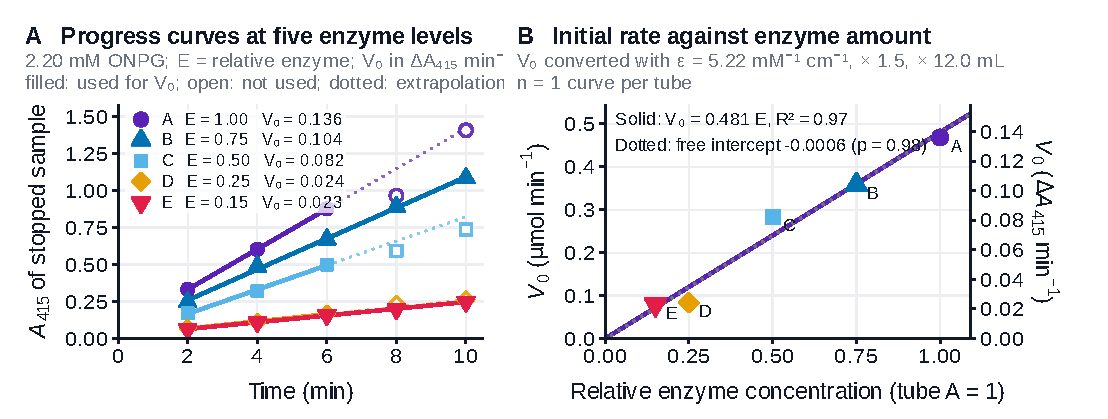
\includegraphics[width=\textwidth]{../../figures/figure2_enzyme_dilution.pdf}
\caption{\textbf{Initial velocity rises approximately in proportion to the amount of β-galactosidase}\newline
(A) Progress curves (\Aa{} of 2.0 mL aliquots stopped with 1.0 mL 1 M Na\textsubscript{2}CO\textsubscript{3}) for 2.20 mM ONPG hydrolyzed by 1.00, 0.75, 0.50, 0.25, and 0.15 relative amounts of the standardized enzyme (tubes A\dash E). Lines are least-squares fits to the initial linear window chosen by the operational rule (STAR Methods); filled points were used, open points (8 min of tubes A and C, below the initial trend) were excluded, dotted lines extrapolate; \Vo{} values are given in the text.\newline
(B) \Vo{} in µmol ONP \permin{} per 12.0 mL assay (× 3.447 from \dAa{} \permin) against relative enzyme; letters identify the tubes. Line, proportional model through the origin, \Vo{} = 0.481 × \textit{E} (\Rsq{} = 0.972); a free-intercept fit (intercept -0.0006 \umolmin, \textit{p} = 0.98) coincides with it and is not drawn. \textit{n} = 1 curve per tube; reference dataset, Part II.}
\end{figure*}

\subsection{β-Galactosidase approaches saturation with ONPG}
Without inhibitor, only the 2.20 mM tube remained linear to 10 min (\Vo{} = 0.132 \dAa{} \permin); in tubes B\dash F the later increments fell below the first, so no linear window could be fitted and \Vo{} was taken as the origin-assumed 0\dash 2 min average rate, \Aa(2 min)/2 min with \Aa{} = 0 assumed at t = 0 (†; Figure 3A; Tables S2 and S3). \Vo{} rose 5.6-fold, from 0.081 to 0.455 \umolmin, over the 32-fold substrate range and flattened above 1 mM (Figure 4A). The Lineweaver\dash Burk regression, 1/\Vo{} = 0.658(1/[S]) + 2.097 (\Rsq{} = 0.928; Figure 4B), gave \Vmax{} = 0.477 \umolmin{} and \Km{} = 0.31 mM; direct nonlinear least squares on the velocity scale gave \Km{} = 0.36 ± 0.13 mM and \Vmax{} = 0.494 ± 0.059 \umolmin{} (Table 1). As a sensitivity scenario, setting the t = 0 absorbance of those tubes to the median intercept of the curves that were linear (0.013 A; range -0.020 to 0.059 A) lowers each 0\dash 2 min estimate by about 0.006 \dAa{} \permin{} and moves \Km{} to 0.55 mM (Lineweaver\dash Burk) or 0.52 mM (nonlinear) (Table S5); intercepts of other reactions do not bound the baseline of these tubes, so the scenario is a what-if calculation, not an uncertainty interval.

\begin{figure*}[!tb]
\centering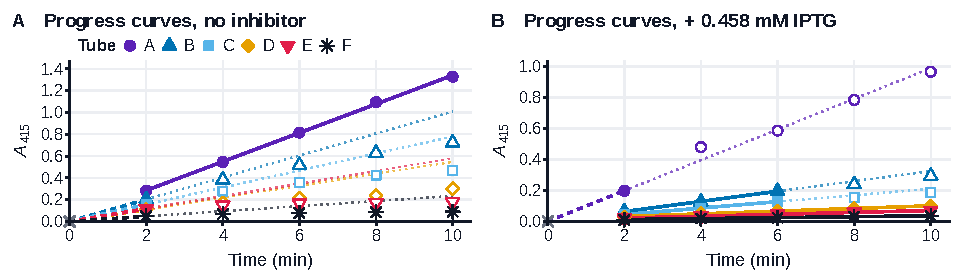
\includegraphics[width=\textwidth]{../../figures/figure3_substrate_saturation.pdf}
\caption{\textbf{Product formation slows as substrate falls and when IPTG is present}\newline
(A) Progress curves for 0.2 mL enzyme acting on 2.20, 1.10, 0.55, 0.275, 0.1375, and 0.069 mM ONPG in 12.0 mL Z buffer at room temperature (tubes A\dash F, no inhibitor). Only tube A stayed linear to 10 min (regression over the filled points); in tubes B\dash F the later increments fell below the first, so \Vo{} is the origin-assumed 0\dash 2 min average rate (dashed segment from ×, where \Aa{} = 0 is assumed at t = 0 because no reading exists), an average over the first interval rather than a measured instantaneous rate; later points (open) were not used; dotted lines extrapolate the fits.\newline
(B) The same six tubes with 0.458 mM IPTG (1.0 mL of 5.5 mM IPTG per 12.0 mL), on a smaller absorbance scale. Tube A is origin-assumed (its 4\dash 10 min increments fell below the first); tubes B\dash F were fitted by regression over the filled points. \Vo{} values are listed in Table S3. \textit{n} = 1 curve per tube; reference dataset, Part III.}
\end{figure*}

\subsection{IPTG raises the apparent \Km{} and inhibits most at low substrate}
With 0.458 mM IPTG, every tube was slower (Figure 3B): by 25\% at 2.20 mM ONPG, 68\% at 1.10 mM, and 87\% at 0.069 mM, so inhibition grew as substrate fell (Figure 4A; Table S3). The Lineweaver\dash Burk line steepened 9.5-fold, 1/\Vo{} = 6.24(1/[S]) + 3.55 (\Rsq{} = 0.988), giving \Kmapp{} = 1.76 mM (5.6-fold increase) and \Vmaxapp{} = 0.282 \umolmin{} (Figure 4B; Table 1). The inhibited velocities halved with each halving of substrate from tube B downward and no plateau was reached within the tested range, so \Vmaxapp{} rests on an extrapolated intercept (3.55 ± 2.33) and a nonlinear fit of the inhibited series alone ran to the \Km{} bound. The independently fitted \Vmaxapp{} is 0.59 of the uninhibited \Vmax, but the data cannot establish whether \Vmax{} changed. The competitive relation gives \Ki{} = [I]/(\Kmapp/\Km{} − 1) = 0.458/(1.76/0.31 − 1) = 0.100 mM.

To compare mechanisms on equal terms, three models were fitted to both series at once (Table 1; Table S6). A competitive model (shared \Vmax, \Km{} raised by 1 + [I]/\Ki) gave \Vmax{} = 0.53 ± 0.07 \umolmin, \Km{} = 0.44 ± 0.17 mM, and \Ki{} = 0.107 ± 0.042 mM (Figure 4A, solid curves). A pure noncompetitive model with the same number of parameters (shared \Km, \Vmax{} reduced by 1 + [I]/\Ki) left a residual sum of squares 1.9 times larger (ΔAIC = 7.8), and a mixed model reduced to the competitive one (its uncompetitive constant ran to the bound of 500 mM). The equal \Vmax{} of the competitive and mixed fits is an assumption of those models rather than an observation; what the data show is that the competitive model describes the twelve points better than the noncompetitive alternative.

\begin{figure*}[!tb]
\centering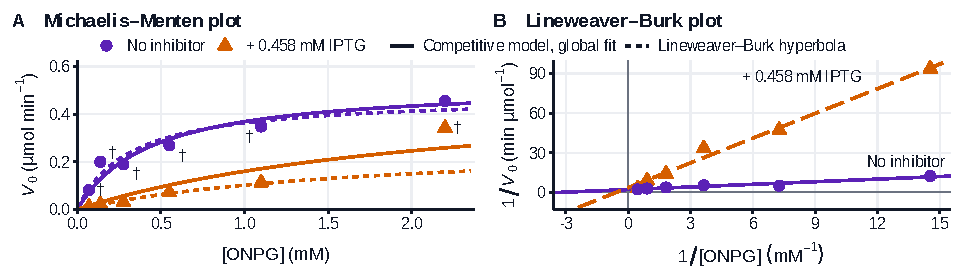
\includegraphics[width=\textwidth]{../../figures/figure4_iptg_inhibition.pdf}
\caption{\textbf{β-Galactosidase approaches saturation with ONPG, and IPTG raises the apparent \Km{}}\newline
(A) \Vo{} against [ONPG] without inhibitor (circles) and with 0.458 mM IPTG (triangles), from the progress curves in Figure 3 (tubes A\dash F). Solid curves, a single competitive-inhibition model fitted to both series at once; dashed curves, hyperbolae implied by the two Lineweaver\dash Burk lines in (B) (shared \Vmax{} = 0.53 ± 0.07 \umolmin, \Km{} = 0.44 ± 0.17 mM, \Ki{} = 0.107 ± 0.042 mM; the shared \Vmax{} is a model assumption). † marks origin-assumed 0\dash 2 min estimates.\newline
(B) Double-reciprocal plot of the same velocities. No inhibitor: 1/\Vo{} = 0.66(1/[S]) + 2.10, \Rsq{} = 0.928, giving \Vmax{} = 0.477 \umolmin{} and \Km{} = 0.31 mM. + IPTG: 1/\Vo{} = 6.24(1/[S]) + 3.55, \Rsq{} = 0.988, giving \Vmaxapp{} = 0.282 \umolmin{} and \Kmapp{} = 1.76 mM. x-intercepts: −1/\Km{} = -3.19 and −1/\Kmapp{} = -0.57 mM\textsuperscript{−1}. \textit{n} = 1 curve per point; reference dataset, Part III.}
\end{figure*}

\begin{table*}[b]
\caption{\textbf{Kinetic parameters of β-galactosidase for ONPG without and with 0.458 mM IPTG}\newline
Reference dataset, tubes A\dash F in every fit; ± values are standard errors of the fit (single measurements, no replicates). Lineweaver\dash Burk is the course method, the nonlinear fits a check; app., apparent value with IPTG; n.d., not determinable (no plateau within 0.069\dash 2.2 mM). \Vmax{} in µmol ONP \permin{} per 12.0 mL assay. \Ki{} from \Kmapp{} = \Km(1 + [I]/\Ki) for the Lineweaver\dash Burk pair and from models fitted to both series with a shared \Vmax{} (competitive) or a shared \Km{} (noncompetitive); RSS, residual sum of squares. –, not applicable.}
\footnotesize
\begin{tabularx}{\textwidth}{@{}llrrrX@{}}
\toprule
Condition & Method & \Km{} (mM) & \Vmax{} (\umolmin) & \Ki{} (mM) & Fit \\
\midrule
No inhibitor & Lineweaver-Burk & 0.314 & 0.477 & – & R2 0.928 \\
No inhibitor & Nonlinear MM & 0.363 ± 0.128 & 0.494 ± 0.059 & – & R2 0.919 \\
+ 0.458 mM IPTG & Lineweaver-Burk & 1.757 (app.) & 0.282 (app.) & 0.100 & R2 0.988 \\
+ 0.458 mM IPTG & Nonlinear MM & n.d. & n.d. & – & R2 0.962 \\
Both series & Global, competitive & 0.435 ± 0.166 & 0.529 ± 0.072 & 0.107 ± 0.042 & RSS 0.0194 \\
Both series & Global, noncompetitive & 0.744 ± 0.382 & 0.626 ± 0.139 & 0.433 ± 0.181 & RSS 0.0371 \\
\bottomrule
\end{tabularx}
\end{table*}

\subsection{Our own measurements reproduce the pattern}
The Results above use the reference dataset. Our experimental dataset, recorded on the same instrument and analyzed with the identical rule and units, gave the same picture (Figures S1 and S4; Table S7). The standard tube agreed with the reference series within 5\% (enzyme dilution) and 15\% (substrate series); nonlinear fits gave \Km{} = 0.14 mM and \Vmax{} = 0.41 \umolmin{} without inhibitor, and IPTG raised \Km{} 8.8-fold while \Vmax{} was unchanged (ratio 1.01), with \Ki{} = 0.059 mM. Two tubes deviated. The inhibited tube nominally containing 1.10 mM ONPG ran 1.57-fold faster than tube A at half the substrate, which no kinetic mechanism permits at fixed enzyme, and 3.7-fold faster than the reference tube B; its profile matches an uninhibited high-substrate tube, consistent with IPTG omitted or ONPG or enzyme over-pipetted (hypotheses, not findings). Its values are retained as recorded and the tube is excluded from fits; including it gives \Kmapp{} = 38 mM. The inhibited 0.1375 mM tube was discarded before measurement.

\subsection{The conclusions that survive alternative estimators, and those that do not}
Because the choice of initial-rate window drives \Km, every parameter was recomputed under five estimators (Figure S3; Table S5): all five points of every curve, the initial-window regression for every curve, the origin-assumed 0\dash 2 min average rate for every curve, the rule under the baseline-offset scenario, and the rule as used. Regression alone gives a negative Lineweaver\dash Burk intercept for the uninhibited series (non-physical), and all five points give \Km{} = 3.4 mM, because both average over the falling phase of the curved low-substrate tubes; the 0\dash 2 min average rate applied to every curve collapses \Kmapp{} to 0.62 mM and raises \Ki{} to 0.50 mM, because for the inhibited tubes, which were linear over 2\dash 10 min, it replaces a five-point regression with a single interval; the offset scenario moves \Ki{} to 0.22 mM. Saturation with substrate and inhibition that grows as substrate falls survive every estimator; the numerical \Km{} (0.31\dash0.55 mM among the rule-based estimators and the global fit) and \Ki{} (0.10\dash0.22 mM among those; 0.50 mM under the uniform 0\dash 2 min estimate) do not; these are alternative method-dependent estimates, not confidence intervals.

\section{Discussion}
What the reference measurements demonstrate directly is that the velocity of β-galactosidase rose with the amount of enzyme and saturated with ONPG, and that IPTG inhibited the enzyme most where substrate was lowest, raising the apparent \Km{} 5.6-fold. What rests on a model is the mechanism: a competitive model described both series better than a pure noncompetitive one with the same number of parameters, and letting IPTG also bind the enzyme\dash substrate complex gained nothing, so the behaviour is consistent with competitive inhibition. It is not a proof. The inhibited series never approached saturation, so its independently fitted \Vmaxapp{} (0.59 of the uninhibited value) is an extrapolation that cannot show whether \Vmax{} changed, and the competitive model shares \Vmax{} by construction, so its fit cannot show that \Vmax{} was unchanged. \Ki{} is 0.10 mM from the Lineweaver\dash Burk pair, 0.11 mM from the global fit, 0.22 mM under the baseline-offset scenario and 0.50 mM if every curve is reduced to its 0\dash 2 min average rate: alternative method-dependent estimates rather than a confidence interval, which place \Ki{} between 0.1 and 0.5 mM under the tested conditions; the 0.08 mM measured for the purified enzyme with ONPG in TES buffer with 145 mM NaCl and 0.01 mM Mg\textsuperscript{2+} at pH 7.0 and 25 °C\cit{10} is of the same order, under conditions (10 mM K\textsuperscript{+}, 1 mM Mg\textsuperscript{2+} in Z buffer here) that were not expected to give identical values. The structural picture predicts this behaviour: IPTG occupies the galactose subsite as a dead-end thiogalactoside and is displaced by substrate.\cit{6}

\Km{} (0.31\dash0.55 mM) is two to five times the 0.12 mM reported for the purified enzyme,\cit{10} and several factors may contribute: five of the six uninhibited \Vo{} values are origin-assumed 0\dash 2 min average rates, which understate the initial rate if it was already falling within that interval and so inflate 1/\Vo{} at low [S] and \Km; the assay conditions (Z buffer, ambient temperature) differ from the literature assay; 2-min manual sampling limits the resolution of fast early phases; and the effective ONPG concentrations in the most dilute tubes carry pipetting and stock uncertainty. With 2-min sampling, the kinetic constants of a fast enzyme are only as good as the rule used to define the initial rate, which is why we state that rule, examine its origin assumption and report every alternative. The deceleration itself is not explained. Those curves flattened at about 38\% of the nominal product yield in tubes E and F (Table S4), which substrate depletion alone does not explain; the timing of the first aliquots, reaction preparation, a lower-than-nominal effective ONPG concentration, stopping and read-out effects could each contribute, and the data do not single one out. The ONPG hypothesis is testable by measuring the stock's own absorbance or by complete hydrolysis of an aliquot. The calibration was not the limiting step: it was linear over five standards (\Rsq{} = 0.9988); the one excluded standard read 0.06\% transmittance near the instrument's linear limit and deviated upward, so its cause is undetermined, and its inclusion would have changed \Vmax{} by 13\% at most and \Km{} and \Ki{} not at all. The standards and the stopped samples share the alkaline matrix, but the kinetic blank was Z buffer alone; the small positive intercepts of the linear curves measure any residual mismatch.

Our experimental dataset reproduced the kinetic pattern with a \Km{} (0.14 mM) closer to the literature value, because our low-substrate tubes stayed linear longer than the reference tubes. Its two deviating tubes illustrate the value of recording everything: the anomalous inhibited tube B is reported with its raw values and excluded only from the fits, with the consequence of including it quantified, and the discarded tube E is left missing rather than estimated. Improvements would be 30-s sampling or continuous monitoring during the first 2 min, substrate concentrations from 0.03 mM to well above 2 mM so that both series approach saturation, duplicate tubes, and spectrophotometric verification of the ONPG stock.

Biologically, the inducer of the \lac{} operon also competes with substrates at the active site of the enzyme it induces, and the same principle, a stable substrate analog that raises the substrate requirement without lowering catalytic capacity, defines competitive drugs from statins to protease inhibitors.

\subsection{Limitations of the study}
Each condition was measured once, so no replicate variance is available and the standard errors quoted come from single regressions. Manual 2-min sampling cannot resolve the initial rate when it falls within the first interval, which affected five of six uninhibited reference tubes; the 0\dash 2 min estimates for those tubes rest on an assumed zero absorbance at t = 0 that was examined in a sensitivity scenario but cannot be verified from these data. The substrate range reached only 2.2 mM, below the apparent \Km{} with IPTG, so the inhibited plateau was never observed and \Vmaxapp{} is extrapolated; the mechanism is inferred from model comparison on twelve single measurements. Read-out resolution (0.001 \textit{A}) is coarse relative to the 0.005 \textit{A} increments of the most dilute inhibited tubes. The plateaus of the low-substrate reference curves suggest that nominal ONPG concentrations may have been lower than stated. Temperature was ambient and not controlled. Literature values were measured in a different buffer by a continuous assay, so exact agreement is not expected.

\section{STAR\starsym Methods}
\subsection{Key resources table}
See Table 2.
\begin{table*}[!tb]
\caption{\textbf{Key resources table}}
\footnotesize
\begin{tabularx}{\textwidth}{@{}Xll@{}}
\toprule
\textbf{REAGENT or RESOURCE} & \textbf{SOURCE} & \textbf{IDENTIFIER} \\
\midrule
\multicolumn{3}{@{}l}{\cellcolor{lav}\textbf{Chemicals, peptides, and recombinant proteins}} \\
β-Galactosidase (\ecoli), standardized solution & B241 teaching laboratory & N/A \\
\textit{o}-Nitrophenyl-β-D-galactopyranoside (ONPG), 3.3 mM & B241 teaching laboratory & N/A \\
Isopropyl-β-D-thiogalactopyranoside (IPTG), 5.5 mM & B241 teaching laboratory & N/A \\
\textit{o}-Nitrophenol (ONP), 1 mM & B241 teaching laboratory & N/A \\
Sodium carbonate, 1 M & B241 teaching laboratory & N/A \\
Z buffer (phosphate, KCl, MgSO\textsubscript{4}, β-mercaptoethanol; pH 7.0) & B241 teaching laboratory & N/A \\
\multicolumn{3}{@{}l}{\cellcolor{lav}\textbf{Deposited data}} \\
Reference dataset (course-provided Part I and Part III measurements) & B241 teaching staff (e-mail of 13 Sep 2026) & \texttt{data/raw/reference/} \\
Experimental dataset (our 14 instrument printouts, transcribed) & This report & \texttt{data/raw/experimental/}; \texttt{report/raw\_data\_printouts/} \\
Processed data, tables, figures & This report & \texttt{data/processed/}, \texttt{tables/}, \texttt{figures/} \\
\multicolumn{3}{@{}l}{\cellcolor{lav}\textbf{Software and algorithms}} \\
R 4.3.3 & R Core Team & https://www.r-project.org \\
tidyverse & Wickham et al.\cit{12} & https://www.tidyverse.org \\
broom, patchwork, scales, here & CRAN & https://cran.r-project.org \\
Analysis scripts (\texttt{R/00\_setup.R} to \texttt{R/09\_graphical\_abstract.R}, \texttt{R/run\_all.R}) & This report & Repository, \texttt{R/} \\
\multicolumn{3}{@{}l}{\cellcolor{lav}\textbf{Other}} \\
GENESYS 10S UV-Vis spectrophotometer & Thermo Fisher Scientific\cit{13} & N/A \\
\bottomrule
\end{tabularx}
\end{table*}

\subsection{Resource availability}
\subsubsection{Lead contact}
Further information and requests should be directed to the lead contact, Almokhtar Aljarodi (almokhtaraljarodi@gmail.com).
\subsubsection{Materials availability}
This study did not generate new unique reagents.
\subsubsection{Data and code availability}
All raw absorbance values (the reference dataset as transcribed from the course's files, and our 14 printouts transcribed and verified value by value), the processed data, every table and figure, and the R scripts that regenerate them are in the public repository \url{https://github.com/almokhtar8-stack/exp2}. \texttt{Rscript R/run\_all.R} reproduces every number in this manuscript; the text itself is filled from the processed outputs so that prose and data cannot disagree. Any additional information is available from the lead contact upon request.

\subsection{Experimental model and study participant details}
No organisms, cell lines, or human participants were used. The enzyme was \Ecoli{} β-galactosidase (EC 3.2.1.23) supplied by the course as a solution standardized to give \Aa{} = 1.20\dash 1.30 after 10 min in the standard reaction (0.2 mL enzyme, 2.20 mM ONPG, 12.0 mL).

\subsection{Method details}
\subsubsection{Datasets}
Two datasets were analyzed: a course-provided reference dataset supplied by the laboratory instructor (Professor Samah Gadhoum; Parts I/II on 10 September 2026 and Part III on 13 September 2026, with the instruction to use them for the Results section) and an experimental dataset collected by our laboratory group on 7 September 2026 (Part II, tubes A\dash E) and 11 September 2026 (Part III, tubes A\dash E without IPTG, A\dash D with IPTG; tube F not performed, inhibited tube E discarded before measurement). The reference measurements were used for the primary kinetic analysis; our experimental measurements were analyzed identically and examined separately for technical interpretation and troubleshooting. The labels describe origin and analytical role, not accuracy or publication status, and the two datasets are not replicates of each other. Reference values were transcribed from the course's .docx and .pptx files and cross-checked value by value against the course's CSV files; the enzyme-dilution table absent from the CSV was transcribed from the .docx. No missing value was estimated.
\subsubsection{Reagents}
Z buffer contained 0.06 M Na\textsubscript{2}HPO\textsubscript{4}, 0.04 M NaH\textsubscript{2}PO\textsubscript{4}, 0.01 M KCl, 0.001 M MgSO\textsubscript{4}, and 0.05 M β-mercaptoethanol, pH 7.0. Stocks were ONPG at 1.0 mg mL\textsuperscript{−1} (3.3 mM), IPTG at 1.31 mg mL\textsuperscript{−1} (5.5 mM), ONP at 1 mM, and Na\textsubscript{2}CO\textsubscript{3} at 1 M. All procedures followed the Experiment 2 laboratory manual\cit{11} except as noted.
\subsubsection{Absorption spectrum and standard curve}
The spectrum of 1.0 mL of 1 mM ONP in 1.0 mL Z buffer and 1.0 mL 1 M Na\textsubscript{2}CO\textsubscript{3} (0.333 mM ONP) was read from 465 to 385 nm in 5 nm steps against the blank (2.0 mL Z buffer + 1.0 mL Na\textsubscript{2}CO\textsubscript{3}). Standards contained 0.25, 0.50, 0.75, 1.0, 1.3, and 1.6 mL of 1 mM ONP made up to 2.0 mL with Z buffer plus 1.0 mL 1 M Na\textsubscript{2}CO\textsubscript{3} ([ONP] = 1 mM × \textit{V}/3.0 mL) and were read at 415 nm; the manual's 2.0 mL standard has no reported reading (Table S1).
\subsubsection{Enzyme dilution}
Five 12.0 mL reactions contained 8.0 mL of 3.3 mM ONPG (2.20 mM), Z buffer, and 0.20, 0.15, 0.10, 0.05, or 0.03 mL of enzyme (relative enzyme 1.00, 0.75, 0.50, 0.25, 0.15), enzyme added last to start the timer.
\subsubsection{Substrate series and inhibition}
Twelve 12.0 mL reactions contained 8.0, 4.0, 2.0, 1.0, 0.5, or 0.25 mL of 3.3 mM ONPG ([ONPG] = 2.20, 1.10, 0.55, 0.275, 0.1375, or 0.06875 mM; tubes A\dash F), Z buffer to volume, 0.2 mL enzyme, and either 1.0 mL Z buffer or 1.0 mL of 5.5 mM IPTG ([IPTG] = 0.458 mM).
\subsubsection{Stopped-reaction sampling}
At 2, 4, 6, 8, and 10 min after enzyme addition, 2.0 mL aliquots were transferred to tubes containing 1.0 mL 1 M Na\textsubscript{2}CO\textsubscript{3}, which stops the reaction and develops the \textit{o}-nitrophenolate color, and \Aa{} was read against a Z-buffer blank in a GENESYS 10S UV-Vis spectrophotometer (1 cm path) at room temperature.

\subsection{Quantification and statistical analysis}
\subsubsection{Concentrations}
Reaction concentrations were calculated from stock concentrations and volumes: [ONPG] = 3.3 mM × \textit{V}/12.0 mL; [IPTG] = 5.5 mM × 1.0/12.0 mL; ONP standards 1 mM × \textit{V}/3.0 mL. Every reaction sums to 12.0 mL and every standard to 3.0 mL (checked programmatically).
\subsubsection{Initial velocities}
The manual asks for \Vo{} from the initial linear portion of each progress curve, with the points used identified. One rule, depending only on the shape of each curve, was applied to all 31 progress curves. Tier 1: the least-squares line \Aa{} = \textit{a} + \textit{bt} was fitted to the 2, 4, and 6 min points and extended one point at a time while the next increment lay within 20\% (or 0.010 \textit{A}, whichever is larger) of the increment predicted by the current line; \Vo{} = \textit{b}. Tier 2: when the second and third increments both fell below the first by more than this tolerance, no linear window could be fitted within the sampled interval, and \Vo{} was taken as the average rate over the first interval, \Aa(2 min)/2 min, which assumes \Aa{} = 0 at t = 0 because no reading exists there; this origin-assumed estimate is an average over 0\dash 2 min rather than a measured instantaneous initial velocity, may lie below or above the true \Vo{} depending on the unmeasured early course, and is flagged (†) wherever it appears. Tier 2 applied to 6 of the 17 reference curves (uninhibited B\dash F, inhibited A) and to one of our own curves. As a sensitivity scenario, the intercepts of the 24 curves that were linear (median 0.013 A, range -0.020 to 0.059 A) were used as an assumed t = 0 absorbance for the origin-assumed curves, and this scenario estimator was carried through every analysis; because those intercepts belong to other reactions, the scenario is an assumption transferred between curves, not a measured baseline or a bound. The extinction coefficient was the slope of \Aa{} against [ONP] over the linear region chosen by the same increment rule.
\subsubsection{Units}
\Vo{} in \dAa{} \permin{} was converted to µmol ONP \permin{} per assay as \Vo/ε × 1.5 (2 mL reaction + 1 mL stop reagent) × 12.0 mL (1 \dAa{} \permin{} = 3.447 \umolmin{} per assay); the manual's instruction to divide the slope by ε gives the cuvette rate in mM \permin, and the two volume factors convert it to an amount per minute. \Km{} and \Ki{} do not depend on this factor; \Vmax{} scales with it.
\subsubsection{Kinetic models}
\Km{} and \Vmax{} were obtained from the Lineweaver\dash Burk regression (\Vmax{} = 1/intercept, \Km{} = slope × \Vmax) and by unweighted nonlinear least squares of \Vo{} = \Vmax[S]/(\Km{} + [S]) on the velocity scale (\texttt{nls}, bounded ``port'' algorithm from a grid of starting values; a fit that runs to the \Km{} bound of 100 mM is reported as ``no plateau within the tested range''). \Ki{} was calculated from \Kmapp{} = \Km(1 + [I]/\Ki). Three global models were fitted to both series simultaneously: competitive, \textit{V} = \Vmax[S]/(\Km(1 + [I]/\Ki) + [S]); pure noncompetitive, \textit{V} = \Vmax[S]/((\Km{} + [S])(1 + [I]/\Ki)); and mixed, \textit{V} = \Vmax[S]/(\Km(1 + [I]/\Ki) + [S](1 + [I]/\Kip)); the first two have the same number of parameters and were compared by residual sum of squares and AIC. Reported uncertainties are regression standard errors from single measurements; no replicate statistics are reported.
\subsubsection{Software}
All calculations were performed in R 4.3.3 with tidyverse,\cit{12} broom, patchwork, scales, and here; figures were drawn with ggplot2 at 600 dpi. The scripts, raw data, and outputs are in the repository listed under data and code availability.

\section{Supplemental information}
Supplemental information includes Figures S1\dash S4 and Tables S1\dash S7 (following the references), the reference diagram for the course's Question 1, and the 14 instrument printouts (repository, \texttt{report/raw\_data\_printouts/}).

\section{Acknowledgments}
We thank the B241 teaching staff for the standardized enzyme, for the reference dataset used in the Results, and for supervision during the laboratory sessions.

\section{Author contributions}
Investigation, A.A. and A.K.; formal analysis, software, visualization, and writing, A.A.

\section{Declaration of interests}
The authors declare no competing interests.

\section{References}
{\footnotesize
\begin{enumerate}[leftmargin=14pt,itemsep=2pt,topsep=0pt,label=\arabic*.]
\item Michaelis, L., and Menten, M.L. (1913). Die Kinetik der Invertinwirkung. Biochem. Z. \textit{49}, 333\dash 369.
\item Johnson, K.A., and Goody, R.S. (2011). The original Michaelis constant: translation of the 1913 Michaelis\dash Menten paper. Biochemistry \textit{50}, 8264\dash 8269. https://doi.org/10.1021/bi201284u.
\item Lineweaver, H., and Burk, D. (1934). The determination of enzyme dissociation constants. J. Am. Chem. Soc. \textit{56}, 658\dash 666. https://doi.org/10.1021/ja01318a036.
\item Dowd, J.E., and Riggs, D.S. (1965). A comparison of estimates of Michaelis\dash Menten kinetic constants from various linear transformations. J. Biol. Chem. \textit{240}, 863\dash 869. https://doi.org/10.1016/S0021-9258(17)45254-9.
\item Jacobson, R.H., Zhang, X.-J., DuBose, R.F., and Matthews, B.W. (1994). Three-dimensional structure of β-galactosidase from \textit{E. coli}. Nature \textit{369}, 761\dash 766. https://doi.org/10.1038/369761a0.
\item Juers, D.H., Heightman, T.D., Vasella, A., McCarter, J.D., Mackenzie, L., Withers, S.G., and Matthews, B.W. (2001). A structural view of the action of \textit{Escherichia coli} (\textit{lacZ}) β-galactosidase. Biochemistry \textit{40}, 14781\dash 14794. https://doi.org/10.1021/bi011727i.
\item Miller, J.H. (1972). Experiments in Molecular Genetics (Cold Spring Harbor Laboratory), pp. 352\dash 355.
\item Jacob, F., and Monod, J. (1961). Genetic regulatory mechanisms in the synthesis of proteins. J. Mol. Biol. \textit{3}, 318\dash 356. https://doi.org/10.1016/S0022-2836(61)80072-7.
\item Herzenberg, L.A. (1959). Studies on the induction of β-galactosidase in a cryptic strain of \textit{Escherichia coli}. Biochim. Biophys. Acta \textit{31}, 525\dash 538. https://doi.org/10.1016/0006-3002(59)90029-0.
\item Juers, D.H., Rob, B., Dugdale, M.L., Rahimzadeh, N., Giang, C., Lee, M., Matthews, B.W., and Huber, R.E. (2009). Direct and indirect roles of His-418 in metal binding and in the activity of β-galactosidase (\textit{E. coli}). Protein Sci. \textit{18}, 1281\dash 1292. https://doi.org/10.1002/pro.140.
\item Biological and Environmental Science and Engineering Division, KAUST (2026). Methods in Molecular and Cellular Biology B241 Laboratory Manual, Experiment 2: Studying Enzyme Kinetics using Spectrophotometry, pp. 1\dash 19.
\item Wickham, H., Averick, M., Bryan, J., Chang, W., McGowan, L.D., François, R., Grolemund, G., Hayes, A., Henry, L., Hester, J., Kuhn, M., Pedersen, T.L., Miller, E., Bache, S.M., Müller, K., Ooms, J., Robinson, D., Seidel, D.P., Spinu, V., Takahashi, K., Vaughan, D., Wilke, C., Woo, K., and Yutani, H. (2019). Welcome to the tidyverse. J. Open Source Softw. \textit{4}, 1686. https://doi.org/10.21105/joss.01686.
\item Thermo Fisher Scientific. GENESYS 10S Series UV-Visible Spectrophotometers, product brochure (specifications: photometric linear range up to 3.5 A at 260 nm; accuracy ± 0.005 A at 1.0 A). Available at: https://tools.thermofisher.com/content/sfs/brochures/GENESYS\%2010S.pdf. Accessed October 10, 2026.
\end{enumerate}}

% ------------------------------------------------------------------ supplement
\clearpage
\onecolumn
\section*{Supplemental information}
\noindent{\footnotesize Figures S1\dash S4 and Tables S1\dash S7 supporting the main text. All items are regenerated from the raw data by \texttt{Rscript R/run\_all.R}.}
\setcounter{figure}{0}\renewcommand{\thefigure}{S\arabic{figure}}
\setcounter{table}{0}\renewcommand{\thetable}{S\arabic{table}}

\begin{table}[h]
\caption{\textbf{Mapping of the reported standard-curve readings to the manual's preparations, related to Figure 1}\newline
The course table lists seven readings (tubes 1\dash 7); the manual describes a blank and seven standards. The first reading is the zero-concentration point (confirmed by the instructor); the remaining six follow the manual's standards 1\dash 6, anchored by the spectrum tube. The manual's standard 7 has no reported reading; whether it was unprepared or unreported is unknown.}
\scriptsize
\begin{tabularx}{\textwidth}{@{}llrrrrlX@{}}
\toprule
Reported tube & Manual preparation & ONP 1 mM (mL) & Z buffer (mL) & Na\textsubscript{2}CO\textsubscript{3} (mL) & [ONP] (mM) & \Aa & Basis \\
\midrule
1 & Blank (0 mL ONP) & 0 & 2 & 1 & 0 & 0.000 & Reported as tube 1 with OD 0; the instructor confirmed it is the zero-concentration point (blank-like preparation, read against itself) \\
2 & Standard 1 & 0.25 & 1.75 & 1 & 0.0833 & 0.428 & Next reported reading; mapping consistent with Beer-Lambert ratio A/[ONP] = 5.1 per mM \\
3 & Standard 2 & 0.5 & 1.5 & 1 & 0.1667 & 0.856 & A/[ONP] = 5.1 per mM \\
4 & Standard 3 & 0.75 & 1.25 & 1 & 0.25 & 1.240 & A/[ONP] = 5.0 per mM \\
5 & Standard 4 & 1 & 1 & 1 & 0.3333 & 1.723 & Identical to the spectrum reading of manual tube 4 at 415 nm (1.723), which anchors the mapping \\
6 & Standard 5 & 1.3 & 0.7 & 1 & 0.4333 & 2.256 & A/[ONP] = 5.2 per mM \\
7 & Standard 6 & 1.6 & 0.4 & 1 & 0.5333 & 3.236 & A/[ONP] = 6.1 per mM; highest reported reading \\
not reported & Standard 7 & 2 & 0 & 1 & 0.6667 & none & Not in the reported table (0.667 mM); unknown whether this standard was not prepared or not reported \\
\bottomrule
\end{tabularx}
\end{table}

\begin{figure}[h]
\centering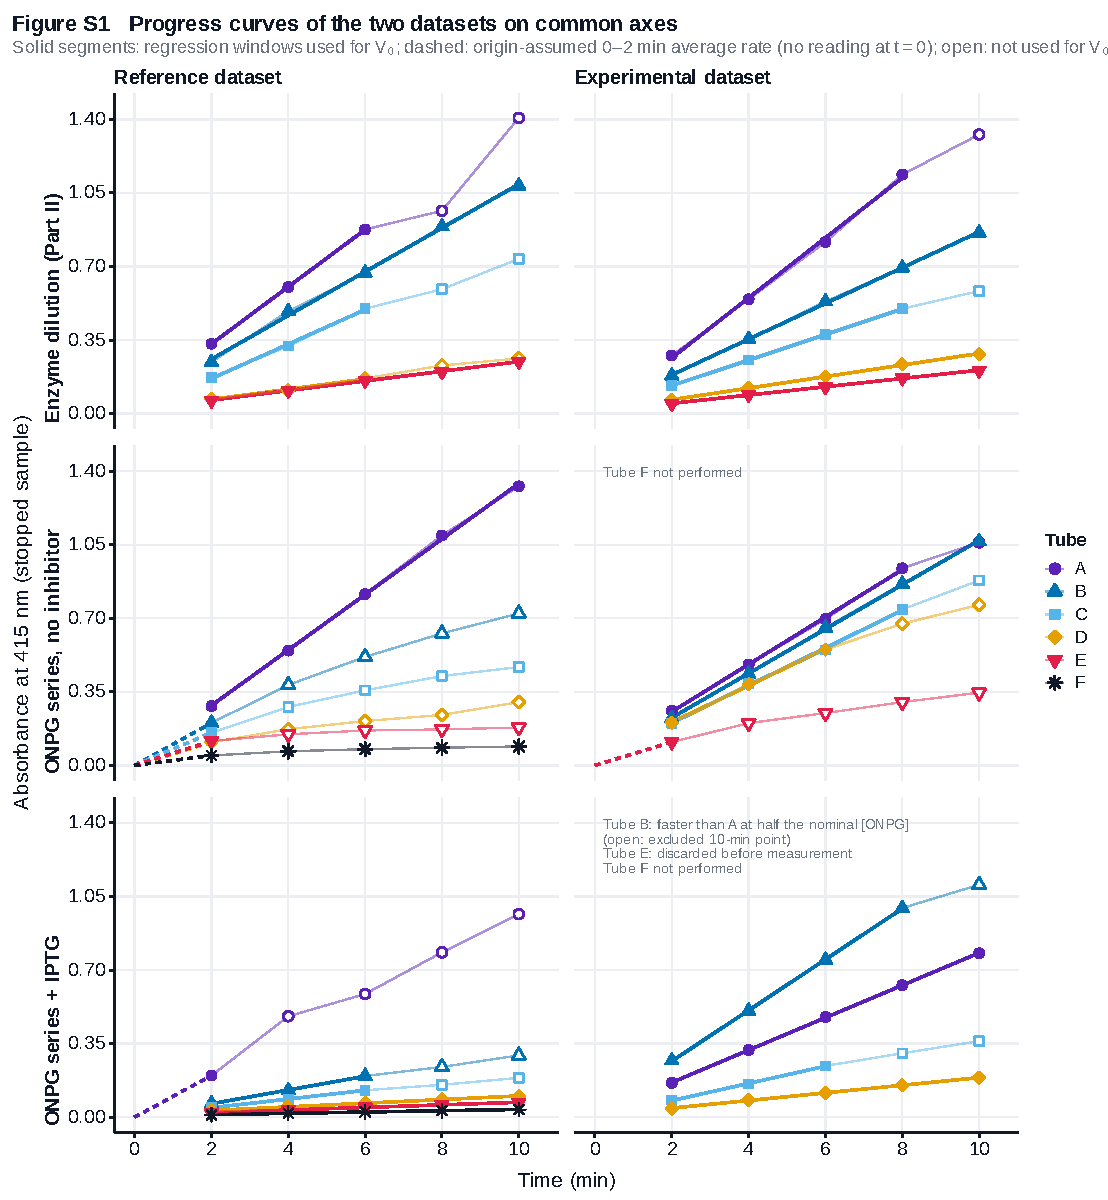
\includegraphics[width=0.95\textwidth]{../../figures/supplementary/figureS1_experimental_vs_reference_curves.pdf}
\caption{\textbf{Progress curves of the two datasets on common axes, related to Figures 2\dash 4}\newline
Reference dataset (left column) and experimental dataset (right column; our 14 GENESYS 10S printouts, 7 and 11 September 2026) for the three experiments. Solid segments are the regression windows and dashed segments the origin-assumed 0\dash 2 min average rates used for \Vo{} under the identical rule. The standard tube (A: 0.2 mL enzyme, 2.20 mM ONPG) agreed between the two datasets within 5\% (enzyme dilution) and 15\% (substrate series). Our low-substrate tubes without inhibitor stayed linear longer than the reference tubes (only tube E was non-linear from the outset), and our inhibited tubes C and D ran about twice as fast as the reference tubes. Our inhibited tube B (open) ran faster than tube A at half the nominal substrate and is excluded from kinetic fits; our inhibited tube E has no data (sample discarded); tube F was not performed on either day.}
\end{figure}

\clearpage
\begin{figure}[h]
\centering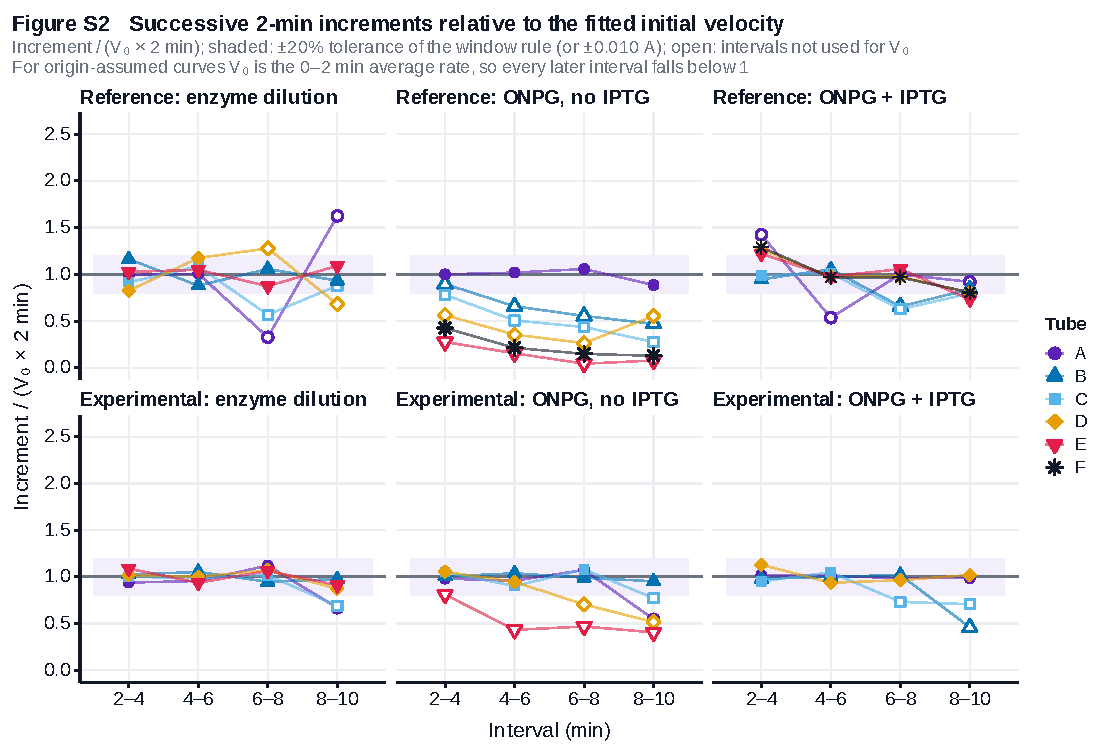
\includegraphics[width=0.95\textwidth]{../../figures/supplementary/figureS2_increment_diagnostics.pdf}
\caption{\textbf{Increment diagnostics behind every \Vo{} decision, related to STAR Methods}\newline
For each of the 31 measured curves, every successive 2-min increment divided by the increment predicted by the fitted \Vo{} (\Vo{} × 2 min). A value of 1 means the interval ran at the fitted initial rate; the shaded band is the acceptance window of the rule (±20\% or ±0.010 \textit{A}, whichever is larger). Open symbols are intervals not used for \Vo. For curves with no initial linear portion (reference no-IPTG B\dash F, reference +IPTG A, experimental no-IPTG E) the reference \Vo{} is the origin-assumed 0\dash 2 min average rate, so all later intervals fall below 1, showing how the measured increments declined: to 35\dash 60\% of the first-interval rate by the second interval in the reference uninhibited tubes B\dash F.}
\end{figure}

\begin{figure}[h]
\centering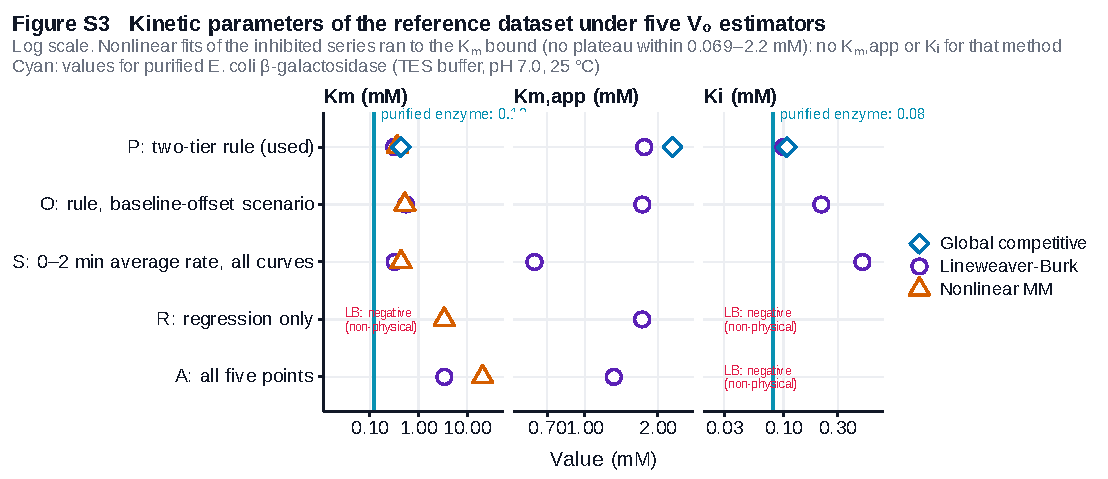
\includegraphics[width=0.95\textwidth]{../../figures/supplementary/figureS3_estimator_sensitivity.pdf}
\caption{\textbf{Sensitivity of the kinetic parameters to the initial-velocity estimator, related to Figures 3 and 4}\newline
\Km{} (no inhibitor), \Kmapp{} (+IPTG), and \Ki{} from the reference dataset under five ways of estimating \Vo: A, all five points of every curve; R, the initial-window regression for every curve; S, the origin-assumed 0\dash 2 min average rate for every curve; O, the two-tier rule under the baseline-offset scenario (t = 0 absorbance set to the median intercept of the linear curves, 0.013 A, an assumption transferred between reactions); P, the two-tier rule used in the Results. Circles, Lineweaver\dash Burk; triangles, nonlinear Michaelis\dash Menten; diamond, global competitive fit. With regression-only \Vo{} the uninhibited Lineweaver\dash Burk line has a negative intercept (non-physical \Km{} and \Vmax, noted in red), and with all five points \Km{} exceeds 3 mM, because both estimators average over the falling phase of the curved low-substrate tubes. The nonlinear +IPTG fits found no plateau within the tested range under any estimator. Cyan lines, \Km{} = 0.12 mM and \Ki{} = 0.08 mM reported for purified \ecoli{} β-galactosidase with ONPG (TES buffer, pH 7.0, 25 °C).\cit{10}}
\end{figure}

\clearpage
\begin{figure}[h]
\centering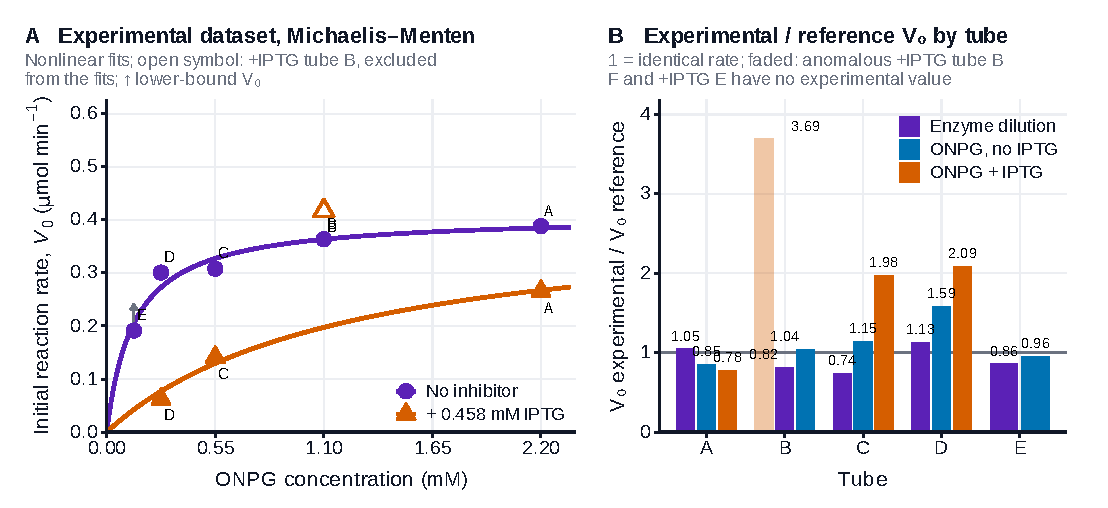
\includegraphics[width=0.95\textwidth]{../../figures/supplementary/figureS4_experimental_kinetics.pdf}
\caption{\textbf{Kinetic analysis of the experimental dataset, related to Figure 4}\newline
(A) Michaelis\dash Menten representation of our Part III data with the same \Vo{} rule and units as the Results, with the anomalous inhibited tube B (open) excluded and the inhibited tube E absent. Nonlinear fits: \Km{} = 0.14 mM, \Vmax{} = 0.41 \umolmin{} without inhibitor; \Kmapp{} = 1.21 mM, \Vmaxapp{} = 0.41 with IPTG (ratio 1.01); \Ki{} = 0.059 mM.\newline
(B) Ratio of our \Vo{} to the reference \Vo{} for every tube measured in both datasets. The standard tube agreed within 5\dash 15\%; our uninhibited tube D and inhibited tubes C and D ran 1.6- to 2.1-fold faster; the anomalous inhibited tube B (faded) ran 3.7-fold faster than the reference tube B.}
\end{figure}

\begin{table}[h]
\caption{\textbf{Primary absorbance data (\Aa) for the substrate series without and with IPTG, related to Figures 3 and 4}\newline
Reference dataset, Part III. Reaction concentrations from the manual's volumes ([ONPG] = 3.3 mM × \textit{V}/12.0 mL; [IPTG] = 5.5 mM × 1.0/12.0 mL). Absorbance of 2.0 mL aliquots stopped with 1.0 mL 1 M Na\textsubscript{2}CO\textsubscript{3}, read at 415 nm.}
\footnotesize
\begin{tabular}{@{}llrrrrrrrr@{}}
\toprule
Condition & Tube & ONPG (mL) & [ONPG] (mM) & [IPTG] (mM) & 2 min & 4 min & 6 min & 8 min & 10 min \\
\midrule
ONPG series, no inhibitor & A & 8 & 2.2 & 0 & 0.282 & 0.546 & 0.815 & 1.094 & 1.328 \\
ONPG series, no inhibitor & B & 4 & 1.1 & 0 & 0.202 & 0.383 & 0.516 & 0.628 & 0.723 \\
ONPG series, no inhibitor & C & 2 & 0.55 & 0 & 0.156 & 0.278 & 0.357 & 0.425 & 0.468 \\
ONPG series, no inhibitor & D & 1 & 0.275 & 0 & 0.11 & 0.172 & 0.211 & 0.24 & 0.301 \\
ONPG series, no inhibitor & E & 0.5 & 0.1375 & 0 & 0.116 & 0.148 & 0.166 & 0.171 & 0.18 \\
ONPG series, no inhibitor & F & 0.25 & 0.06875 & 0 & 0.047 & 0.067 & 0.077 & 0.084 & 0.09 \\
ONPG series + IPTG & A & 8 & 2.2 & 0.458 & 0.198 & 0.48 & 0.586 & 0.784 & 0.966 \\
ONPG series + IPTG & B & 4 & 1.1 & 0.458 & 0.065 & 0.127 & 0.196 & 0.239 & 0.294 \\
ONPG series + IPTG & C & 2 & 0.55 & 0.458 & 0.045 & 0.086 & 0.128 & 0.154 & 0.187 \\
ONPG series + IPTG & D & 1 & 0.275 & 0.458 & 0.029 & 0.051 & 0.068 & 0.085 & 0.099 \\
ONPG series + IPTG & E & 0.5 & 0.1375 & 0.458 & 0.02 & 0.035 & 0.047 & 0.06 & 0.069 \\
ONPG series + IPTG & F & 0.25 & 0.06875 & 0.458 & 0.011 & 0.019 & 0.025 & 0.031 & 0.036 \\
\bottomrule
\end{tabular}
\end{table}

\begin{table}[h]
\caption{\textbf{Initial velocities and reciprocals for the Lineweaver\dash Burk analysis, related to Figure 4}\newline
Reference dataset, Part III. \Vo{} in \dAa{} \permin{} and in µmol ONP \permin{} per assay (× 3.447); 1/[S] in mM\textsuperscript{−1}; 1/\Vo{} in min µmol\textsuperscript{−1}. †, origin-assumed 0\dash 2 min average rate (\Aa{} = 0 assumed at t = 0); other values, regression on the initial linear window.}
\footnotesize
\begin{tabular}{@{}llrrrrrrrrrr@{}}
\toprule
Series & Tube & [S] (mM) & 2 min & 4 min & 6 min & 8 min & 10 min & \Vo{} (\dAa/min) & \Vo{} (µmol/min) & 1/[S] & 1/\Vo \\
\midrule
no inhibitor & A & 2.2 & 0.282 & 0.546 & 0.815 & 1.094 & 1.328 & 0.132 & 0.455 & 0.45 & 2.2 \\
no inhibitor & B & 1.1 & 0.202 & 0.383 & 0.516 & 0.628 & 0.723 & 0.101† & 0.348† & 0.91 & 2.87 \\
no inhibitor & C & 0.55 & 0.156 & 0.278 & 0.357 & 0.425 & 0.468 & 0.078† & 0.269† & 1.82 & 3.72 \\
no inhibitor & D & 0.275 & 0.11 & 0.172 & 0.211 & 0.24 & 0.301 & 0.055† & 0.190† & 3.64 & 5.28 \\
no inhibitor & E & 0.1375 & 0.116 & 0.148 & 0.166 & 0.171 & 0.18 & 0.058† & 0.200† & 7.27 & 5 \\
no inhibitor & F & 0.06875 & 0.047 & 0.067 & 0.077 & 0.084 & 0.09 & 0.0235† & 0.081† & 14.55 & 12.35 \\
+ 0.458 mM IPTG & A & 2.2 & 0.198 & 0.48 & 0.586 & 0.784 & 0.966 & 0.099† & 0.341† & 0.45 & 2.93 \\
+ 0.458 mM IPTG & B & 1.1 & 0.065 & 0.127 & 0.196 & 0.239 & 0.294 & 0.03275 & 0.113 & 0.91 & 8.86 \\
+ 0.458 mM IPTG & C & 0.55 & 0.045 & 0.086 & 0.128 & 0.154 & 0.187 & 0.02075 & 0.072 & 1.82 & 13.98 \\
+ 0.458 mM IPTG & D & 0.275 & 0.029 & 0.051 & 0.068 & 0.085 & 0.099 & 0.0087 & 0.030 & 3.64 & 33.35 \\
+ 0.458 mM IPTG & E & 0.1375 & 0.02 & 0.035 & 0.047 & 0.06 & 0.069 & 0.00615 & 0.021 & 7.27 & 47.18 \\
+ 0.458 mM IPTG & F & 0.06875 & 0.011 & 0.019 & 0.025 & 0.031 & 0.036 & 0.0031 & 0.011 & 14.55 & 93.59 \\
\bottomrule
\end{tabular}
\end{table}

\begin{table}[h]
\caption{\textbf{Substrate converted by 2 and 10 min, related to Discussion}\newline
Percent of nominal ONPG converted to ONP, from \Aa/(ε × 2/3) relative to the nominal reaction concentration, for every curve of both datasets.}
\footnotesize
\begin{tabular}{@{}llrrrrr@{}}
\toprule
Dataset & Tube & [ONPG] (mM) & \Aa{} 2 min & \% converted, 2 min & \Aa{} 10 min & \% converted, 10 min \\
\midrule
Reference Part III (+IPTG) & A & 2.2 & 0.198 & 2.6 & 0.966 & 12.6 \\
Reference Part III (+IPTG) & B & 1.1 & 0.065 & 1.7 & 0.294 & 7.7 \\
Reference Part III (+IPTG) & C & 0.55 & 0.045 & 2.4 & 0.187 & 9.8 \\
Reference Part III (+IPTG) & D & 0.275 & 0.029 & 3 & 0.099 & 10.3 \\
Reference Part III (+IPTG) & E & 0.138 & 0.02 & 4.2 & 0.069 & 14.4 \\
Reference Part III (+IPTG) & F & 0.0687 & 0.011 & 4.6 & 0.036 & 15 \\
Reference Part III (-IPTG) & A & 2.2 & 0.282 & 3.7 & 1.33 & 17.3 \\
Reference Part III (-IPTG) & B & 1.1 & 0.202 & 5.3 & 0.723 & 18.9 \\
Reference Part III (-IPTG) & C & 0.55 & 0.156 & 8.1 & 0.468 & 24.4 \\
Reference Part III (-IPTG) & D & 0.275 & 0.11 & 11.5 & 0.301 & 31.4 \\
Reference Part III (-IPTG) & E & 0.138 & 0.116 & 24.2 & 0.18 & 37.6 \\
Reference Part III (-IPTG) & F & 0.0687 & 0.047 & 19.6 & 0.09 & 37.6 \\
Experimental Part III (+IPTG) & A & 2.2 & 0.163 & 2.1 & 0.78 & 10.2 \\
Experimental Part III (+IPTG) & B & 1.1 & 0.269 & 7 & 1.11 & 28.9 \\
Experimental Part III (+IPTG) & C & 0.55 & 0.08 & 4.2 & 0.362 & 18.9 \\
Experimental Part III (+IPTG) & D & 0.275 & 0.041 & 4.3 & 0.188 & 19.6 \\
Experimental Part III (-IPTG) & A & 2.2 & 0.259 & 3.4 & 1.06 & 13.9 \\
Experimental Part III (-IPTG) & B & 1.1 & 0.224 & 5.8 & 1.06 & 27.8 \\
Experimental Part III (-IPTG) & C & 0.55 & 0.2 & 10.4 & 0.88 & 46 \\
Experimental Part III (-IPTG) & D & 0.275 & 0.202 & 21.1 & 0.764 & 79.8 \\
Experimental Part III (-IPTG) & E & 0.138 & 0.111 & 23.2 & 0.346 & 72.3 \\
\bottomrule
\end{tabular}
\end{table}

\begin{table}[h]
\caption{\textbf{Kinetic parameters under five initial-velocity estimators, related to Figure S3}\newline
Reference dataset. A, all five points of every curve; R, initial-window regression for every curve; S, origin-assumed 0\dash 2 min average rate for every curve; O, the two-tier rule under the baseline-offset scenario; P, the two-tier rule of the Results. Negative values mark non-physical estimates from a negative Lineweaver\dash Burk intercept; –, undefined (nonlinear +IPTG fit ran to the \Km{} bound).}
\scriptsize
\begin{tabular}{@{}llrrrrrrrrrll@{}}
\toprule
Estimator & Method & \Km & \Kmapp & \Vmax & \Vmaxapp & \Kmapp/\Km & \Vmaxapp/\Vmax & \Ki & \Rsq{} (−I) & \Rsq{} (+I) & Physical & Primary \\
\midrule
A & Lineweaver-Burk & 3.405 & 1.317 & 0.849 & 0.214 & 0.39 & 0.25 & -0.747 & 0.965 & 0.988 & TRUE / TRUE & – \\
A & Nonlinear MM & 20.9 & – & 4.744 & – & – & – & – & 0.995 & 0.951 & TRUE / FALSE & – \\
O & Lineweaver-Burk & 0.551 & 1.726 & 0.577 & 0.277 & 3.13 & 0.48 & 0.215 & 0.917 & 0.988 & TRUE / TRUE & – \\
O & Nonlinear MM & 0.524 & – & 0.527 & – & – & – & – & 0.924 & 0.971 & TRUE / FALSE & – \\
P & Lineweaver-Burk & 0.314 & 1.757 & 0.477 & 0.282 & 5.6 & 0.59 & 0.1 & 0.928 & 0.988 & TRUE / TRUE & yes \\
P & Nonlinear MM & 0.363 & – & 0.494 & – & – & – & – & 0.919 & 0.962 & TRUE / FALSE & – \\
R & Lineweaver-Burk & -3.48 & 1.722 & -0.912 & 0.276 & -0.49 & -0.3 & -0.307 & 0.99 & 0.989 & FALSE / TRUE & – \\
R & Nonlinear MM & 3.379 & – & 1.147 & – & – & – & – & 0.998 & 0.972 & TRUE / FALSE & – \\
S & Lineweaver-Burk & 0.322 & 0.62 & 0.487 & 0.188 & 1.93 & 0.39 & 0.495 & 0.928 & 0.984 & TRUE / TRUE & – \\
S & Nonlinear MM & 0.436 & – & 0.537 & – & – & – & – & 0.908 & 0.954 & TRUE / FALSE & – \\
P & Global nonlinear competitive & 0.435 & 2.297 & 0.529 & 0.529 & 5.28 & 1 & 0.107 & 0.919 & – & TRUE / NA & – \\
\bottomrule
\end{tabular}
\end{table}

\begin{table}[h]
\caption{\textbf{Global fits of three inhibition models to both series, related to Figure 4}\newline
Twelve single measurements (six per series). Competitive and pure noncompetitive models have three parameters each; the mixed model has four and nests both.}
\footnotesize
\begin{tabular}{@{}llrrrrrll@{}}
\toprule
Model & Parameter & Estimate & SE & RSS & AIC & n & Converged & Note \\
\midrule
global competitive & Vmax & 0.5285 & 0.072 & 0.01941 & -35.07 & 12 & TRUE & – \\
global competitive & Km & 0.4351 & 0.1662 & 0.01941 & -35.07 & 12 & TRUE & – \\
global competitive & Ki & 0.1071 & 0.0418 & 0.01941 & -35.07 & 12 & TRUE & – \\
global noncompetitive & Vmax & 0.6262 & 0.1388 & 0.03713 & -27.28 & 12 & TRUE & – \\
global noncompetitive & Km & 0.7438 & 0.3824 & 0.03713 & -27.28 & 12 & TRUE & – \\
global noncompetitive & Ki & 0.4333 & 0.1806 & 0.03713 & -27.28 & 12 & TRUE & – \\
global mixed & Vmax & 0.5286 & 0.0778 & 0.01942 & -33.06 & 12 & TRUE & – \\
global mixed & Km & 0.4352 & 0.1788 & 0.01942 & -33.06 & 12 & TRUE & – \\
global mixed & Ki & 0.1072 & 0.0792 & 0.01942 & -33.06 & 12 & TRUE & – \\
global mixed & Kip & 500 & 422500 & 0.01942 & -33.06 & 12 & TRUE & at upper bound (model reduces to competitive) \\
\bottomrule
\end{tabular}
\end{table}

\begin{table}[h]
\caption{\textbf{Kinetics from our own substrate series, related to Figure S4}\newline
Same rule and units as the Results. With the anomalous inhibited tube B excluded, the nonlinear fits show the pattern expected for competitive inhibition (apparent \Vmax{} ratio 1.01, a single-measurement estimate); including it makes the Lineweaver\dash Burk analysis meaningless.}
\footnotesize
\begin{tabular}{@{}llrrrrrrrrl@{}}
\toprule
Inhibited B & Method & \Km{} (mM) & \Kmapp{} (mM) & \Vmax & \Vmaxapp & \Vmaxapp/\Vmax & \Ki{} (mM) & \Rsq{} (−I) & \Rsq{} (+I) & Tubes (−I / +I) \\
\midrule
excluded & Lineweaver-Burk & 0.156 & 3.087 & 0.421 & 0.792 & 1.88 & 0.024 & – & 0.95 & 0.969 & ABCDE / ACD \\
excluded & Nonlinear MM & 0.137 & 1.206 & 0.409 & 0.414 & 1.01 & 0.059 & 0.029 & 0.942 & 0.984 & ABCDE / ACD \\
included & Lineweaver-Burk & 0.156 & 38.16 & 0.421 & 9.042 & 21.5 & 0.002 & – & 0.95 & 0.945 & ABCDE / ABCD \\
included & Nonlinear MM & 0.137 & 0.783 & 0.409 & 0.458 & 1.12 & 0.097 & 0.215 & 0.942 & 0.541 & ABCDE / ABCD \\
excluded & Global nonlinear competitive & 0.137 & 1.179 & 0.409 & 0.409 & 1 & 0.061 & 0.013 & 0.981 & – & ABCDE / ACD \\
included & Global nonlinear competitive & 0.149 & 0.647 & 0.419 & 0.419 & 1 & 0.137 & 0.115 & 0.691 & – & ABCDE / ABCD \\
\bottomrule
\end{tabular}
\end{table}

\end{document}
